\begin{surferIntroPage}{Первые шаги}{tutorial_koord1}{Первые шаги с программой SURFER}
Эта компьютерная программа называется SURFER («сёрфер»). Когда слышат это слово, то думают о солнце, море и волнах. Но это название происходит от английского слова surface, которое в переводе означает «поверхность». При помощи SURFER можно получать изображения. Об алгебраических поверхностях и о том, как работает эта программа, Вы узнаете из введения. Кликните справа, чтобы выбрать один из разделов.
\\
Программа SURFER демонстрируется в рамках выставки IMAGINARY. Она была создана в рамках Года математики в Германии (2008 г.). У истоков выставки стояли специалисты всемирно известного Математического научно-исследовательского института г. Обервольфаха в германском регионе Шварцвальд. В институте каждую неделю проходят конференции, посвященные актуальным научным исследованиям. Эти мероприятия очень важны для того, чтобы учёные со всего мира обменивались мнениями и результатами своей научной работы.
\vspace{-1ex}
\begin{center}
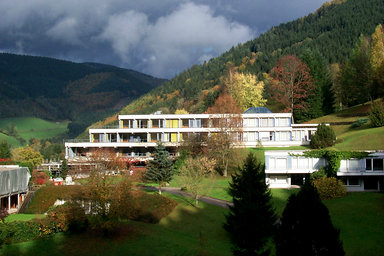
\includegraphics[width=3cm]{./../../common/images/photo_mfo.jpg}
\end{center}
\vspace{-2ex}
SURFER – бесплатное программное обеспечение, которое можно скачать на интернет-сайте выставки
\vspace{-3ex}
\begin{center}
www.imaginary-exhibition.com
\end{center}
\vspace{-2ex}
С правой стороны Вы можете выбрать введение в математический аппарат. Оно начинается с поверхности «Цитрус». С левой стороны Вы можете перейти к другой галерее, например, к галерее фантастических поверхностей.
\end{surferIntroPage}
